%(BEGIN_QUESTION)
% Copyright 2015, Tony R. Kuphaldt, released under the Creative Commons Attribution License (v 1.0)
% This means you may do almost anything with this work of mine, so long as you give me proper credit

A venturi tube is used to measure the flow rate of steam exiting a power boiler:

$$\includegraphics[width=15.5cm]{i04087x01.eps}$$

Supposing this venturi tube normally develops a differential pressure of 100 inches water column at a flow rate of 970 pounds per minute with a steam density of $\rho$ = 1.33 lbm/ft$^{3}$, calculate the following:

\begin{itemize}
\item{} Differential pressure at 700 lbm/min mass flow = \underbar{\hskip 50pt}
\vskip 5pt
\item{} Differential pressure at 550 lbm/min mass flow and $\rho$ = 1.30 lbm/ft$^{3}$ = \underbar{\hskip 50pt}
\vskip 5pt
\item{} Mass flow rate at 90 "W.C. = \underbar{\hskip 50pt}
\vskip 5pt
\item{} Mass flow rate at 43 "W.C. and $\rho$ = 1.35 lbm/ft$^{3}$ = \underbar{\hskip 50pt}
\end{itemize}

\vskip 20pt \vbox{\hrule \hbox{\strut \vrule{} {\bf Suggestions for Socratic discussion} \vrule} \hrule}

\begin{itemize}
\item{} Explain why both steam flow and water flow are best measured in {\it mass} units rather than volumetric in this process application.
\item{} Identify some factors that could realistically cause the steam's density to change.
\end{itemize}

\underbar{file i04087}
%(END_QUESTION)





%(BEGIN_ANSWER)

\noindent
{\bf Partial answer:}

\vskip 10pt

\begin{itemize}
\item{} Differential pressure at 550 lbm/min mass flow and $\rho$ = 1.30 lbm/ft$^{3}$ = \underbar{\bf 32.89 "W.C.}
\item{} Mass flow rate at 90 "W.C. = \underbar{\bf 920 lbm/min}
\end{itemize}


%(END_ANSWER)





%(BEGIN_NOTES)

$$W = k \sqrt{\rho \Delta P}$$

For a mass flow rate of 970 pounds per minute at a differential pressure of 100 "WC and a flowing density of 1.33 pounds per cubic foot, the value of $k$ will be 84.1097.

\begin{itemize}
\item{} Differential pressure at 700 lbm/min mass flow = \underbar{\bf 52.08 "W.C.}
\item{} Differential pressure at 550 lbm/min mass flow and $\rho$ = 1.30 lbm/ft$^{3}$ = \underbar{\bf 32.89 "W.C.}
\item{} Mass flow rate at 90 "W.C. = \underbar{\bf 920.22 lbm/min}
\item{} Mass flow rate at 43 "W.C. and $\rho$ = 1.35 lbm/ft$^{3}$ = \underbar{\bf 640.84 lbm/min}
\end{itemize}










\vfil \eject

\noindent
{\bf Prep Quiz:}

If the volumetric flow rate through a venturi tube suddenly doubles, the differential pressure it produces will:

\begin{itemize}
\item{} Halve (${1 \over 2} \times$) 
\vskip 5pt 
\item{} Remain the same
\vskip 5pt 
\item{} Double (2$\times$)
\vskip 5pt 
\item{} Triple (3$\times$)
\vskip 5pt 
\item{} Quadruple (4$\times$)
\vskip 5pt 
\item{} Increase by 8$\times$ 
\end{itemize}

%INDEX% Measurement, flow: simple ``k'' factor equation for flow/pressure correlation
%INDEX% Process: steam boiler 

%(END_NOTES)


